\begin{centering}
    \subsection{Результаты численных экспериментов}
\end{centering}

Кратко опишем используемые в численных экспериментах тесты.
Детальные формулировки приводились ранее.
\begin{enumerate}
    \item $\varphi^{\text{$\theta$-UMPU}}$ -- РНМН тест уровня 
    $\alpha=0.05$ на нулевое значение параметра: $$\theta = \ln  \left(\dfrac{p_{001}p_{111}p_{010}p_{100}}{p_{011}p_{101}p_{000}p_{110}}\right)$$
    Поскольку из $X \ci Y \mid Z$ следует $\theta=0$, 
    то данный тест является тестом уровня $\alpha=0.05$ для проверки
    гипотезы $H:X \ci Y \mid Z$.
    \item $\varphi^{\text{Partial}}$ -- точный тест уровня $\alpha=0.05$
    на нулевое значение частного коэффициента корреляции
    Пирсона $\rho^{XY\cdot Z}$ для трехмерного нормального распределения.
    В предположении того, что $\varphi^{\text{Partial}}$ также является тестом
    уровня $\alpha=0.05$ в трехмерном распределении Бернулли, 
    этот тест также является тестом уровня $\alpha=0.05$ для проверки
    гипотезы $H:X \ci Y \mid Z$,
    поскольку из $X \ci Y \mid Z$ следует $\rho^{XY\cdot Z}=0$.
\end{enumerate}

\begin{figure}[H]
    \centering
    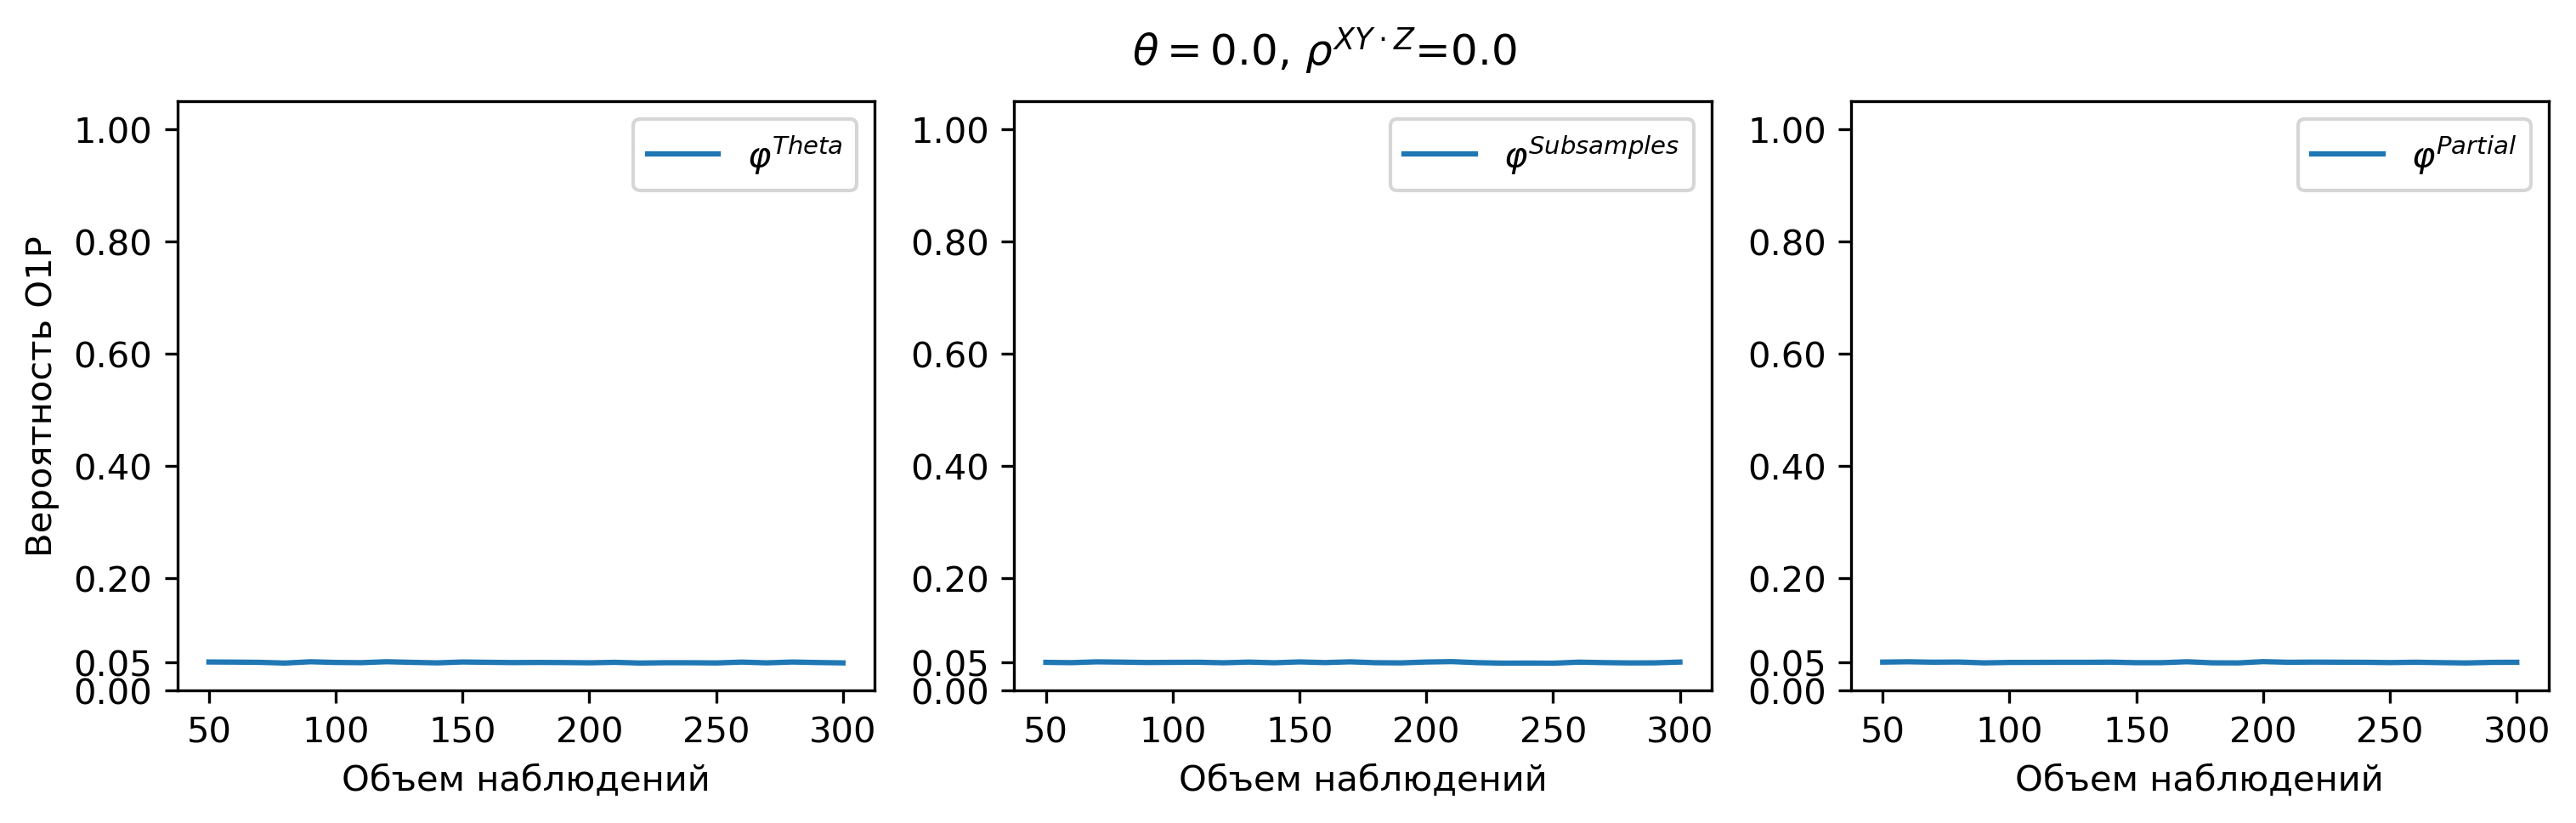
\includegraphics[scale=0.65]{images/graph1.png}
    \caption{Графики зависимости вероятности ошибки 1 рода (О1Р) от количества наблюдений
    на тестах $\varphi^{\text{$\theta$-UMPU}}$, $\varphi^{\text{Subsamples}}$, $\varphi^{\text{Partial}}$
    в трехмерном распределении Бернулли с $p_{000}=0.125, p_{001}=0.125, p_{010}=0.125, p_{011}=0.125,
    p_{100}=0.125, p_{101}=0.125, p_{110}=0.125, p_{111}=0.125$. Вероятности оцениваются по $10^5$ экспериментам.} \label{fig:1}
\end{figure}
    

\begin{figure}[H]
    \centering
    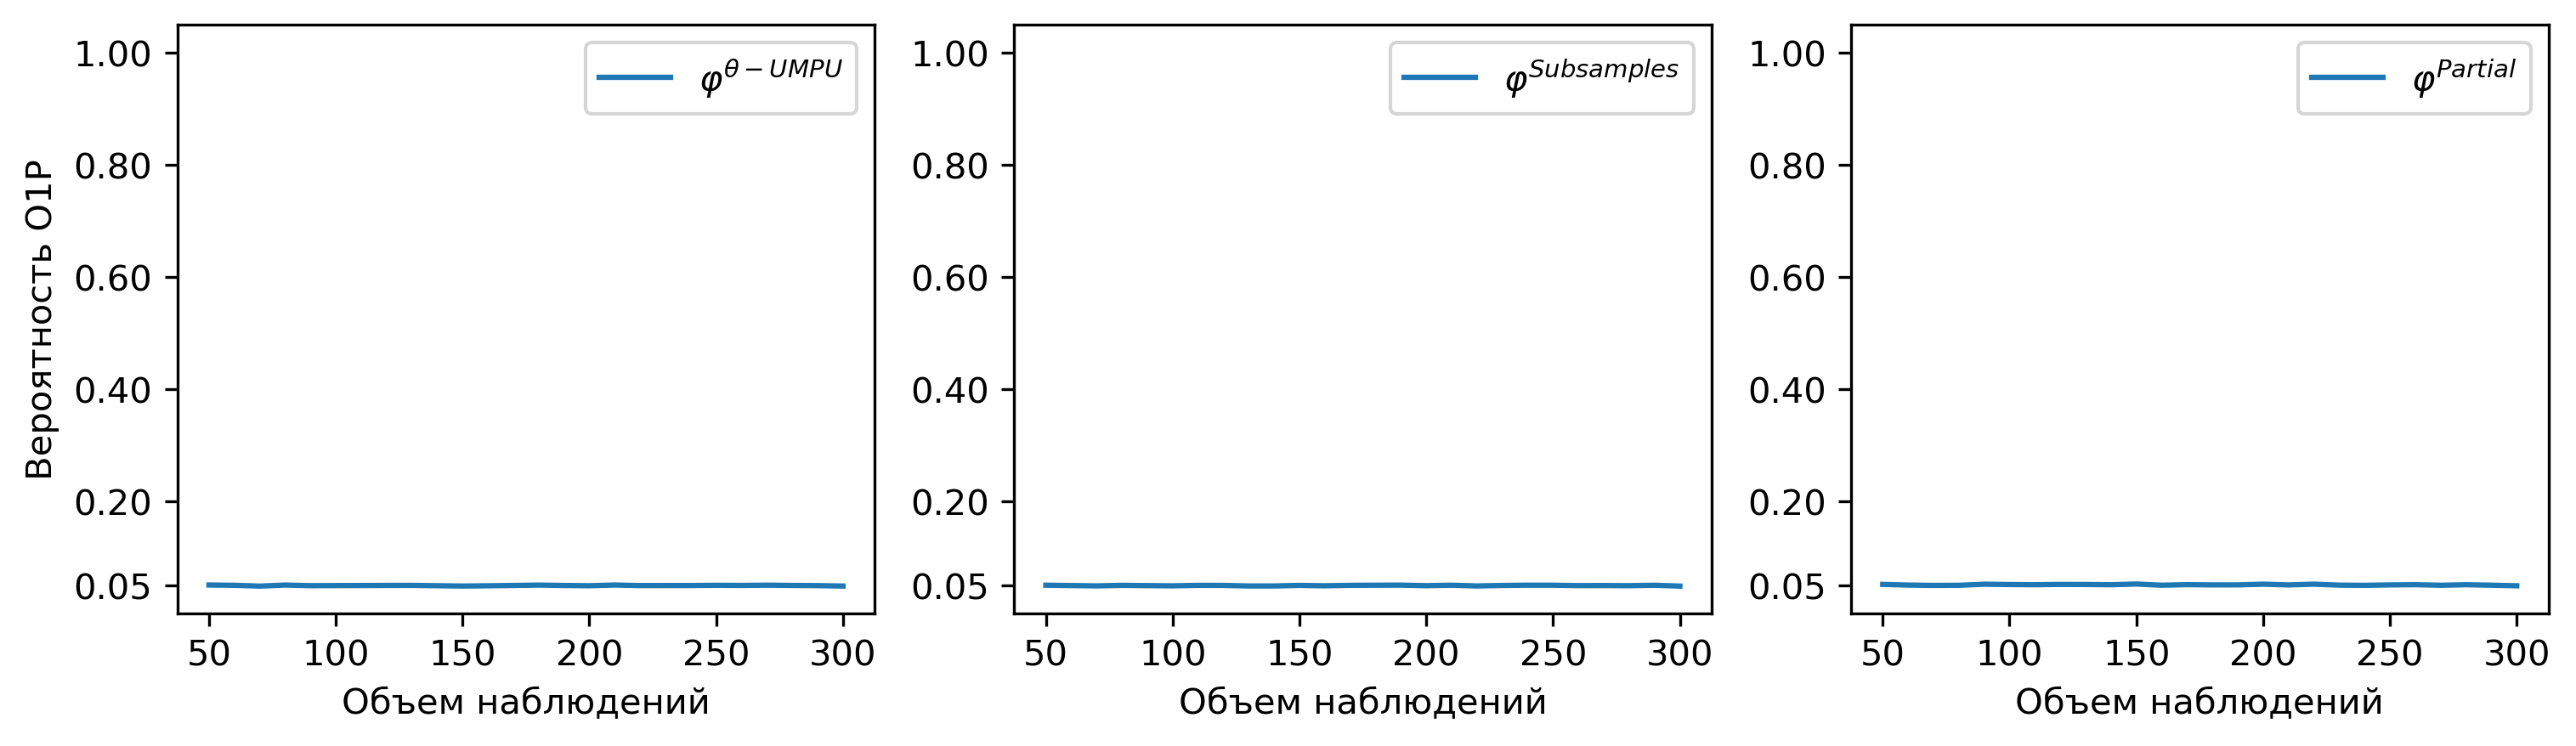
\includegraphics[scale=0.65]{images/graph2.png}
    \caption{Графики зависимости вероятности ошибки 1 рода (О1Р) от количества наблюдений
    на тестах $\varphi^{\text{$\theta$-UMPU}}$, $\varphi^{\text{Subsamples}}$, $\varphi^{\text{Partial}}$
    в трехмерном распределении Бернулли с $p_{000}=0.15, p_{001}=0.1, p_{010}=0.3, p_{011}=0.1,
    p_{100}=0.05, p_{101}=0.1, p_{110}=0.1, p_{111}=0.1$. Вероятности оцениваются по $10^5$ экспериментам.} \label{fig:2}
\end{figure}

\begin{figure}[H]
    \centering
    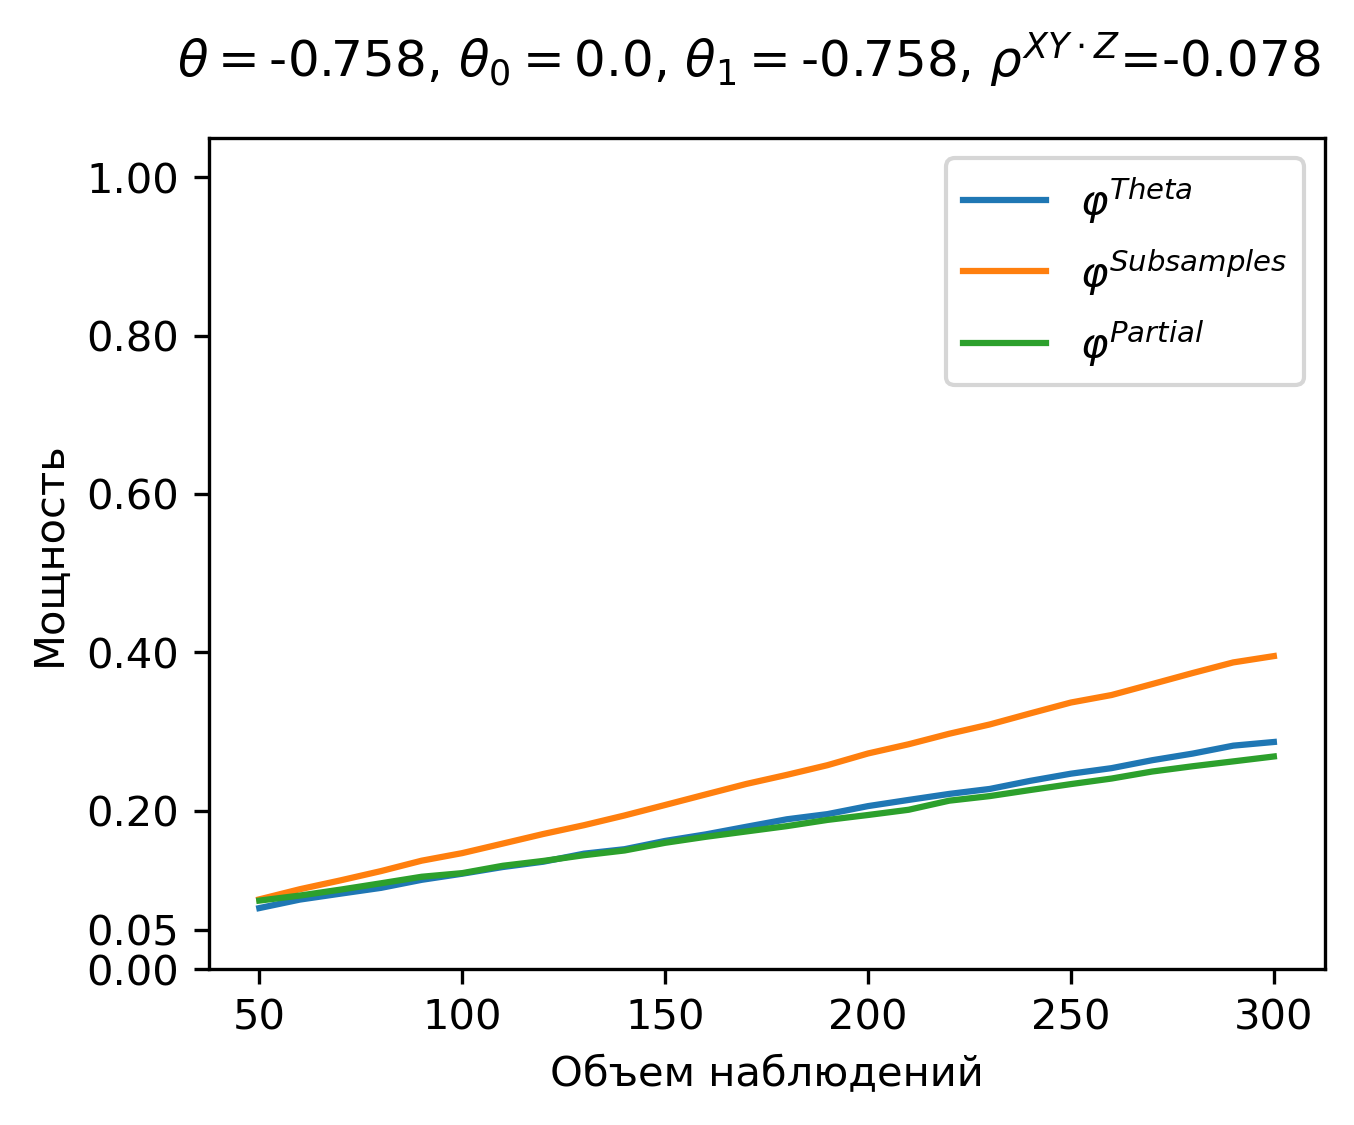
\includegraphics[scale=0.8]{images/graph3.png}
    \caption{Графики зависимости мощности от количества наблюдений
    на тестах $\varphi^{\text{$\theta$-UMPU}}$, $\varphi^{\text{Subsamples}}$, $\varphi^{\text{Partial}}$
    в трехмерном распределении Бернулли с $p_{000}=0.15, p_{001}=0.06, 
    p_{010}=0.3, p_{011}=0.16,
    p_{100}=0.05, p_{101}=0.08, p_{110}=0.1, p_{111}=0.1$. Вероятности оцениваются по $10^5$ экспериментам.} \label{fig:3}
\end{figure}

\begin{figure}[H]
    \centering
    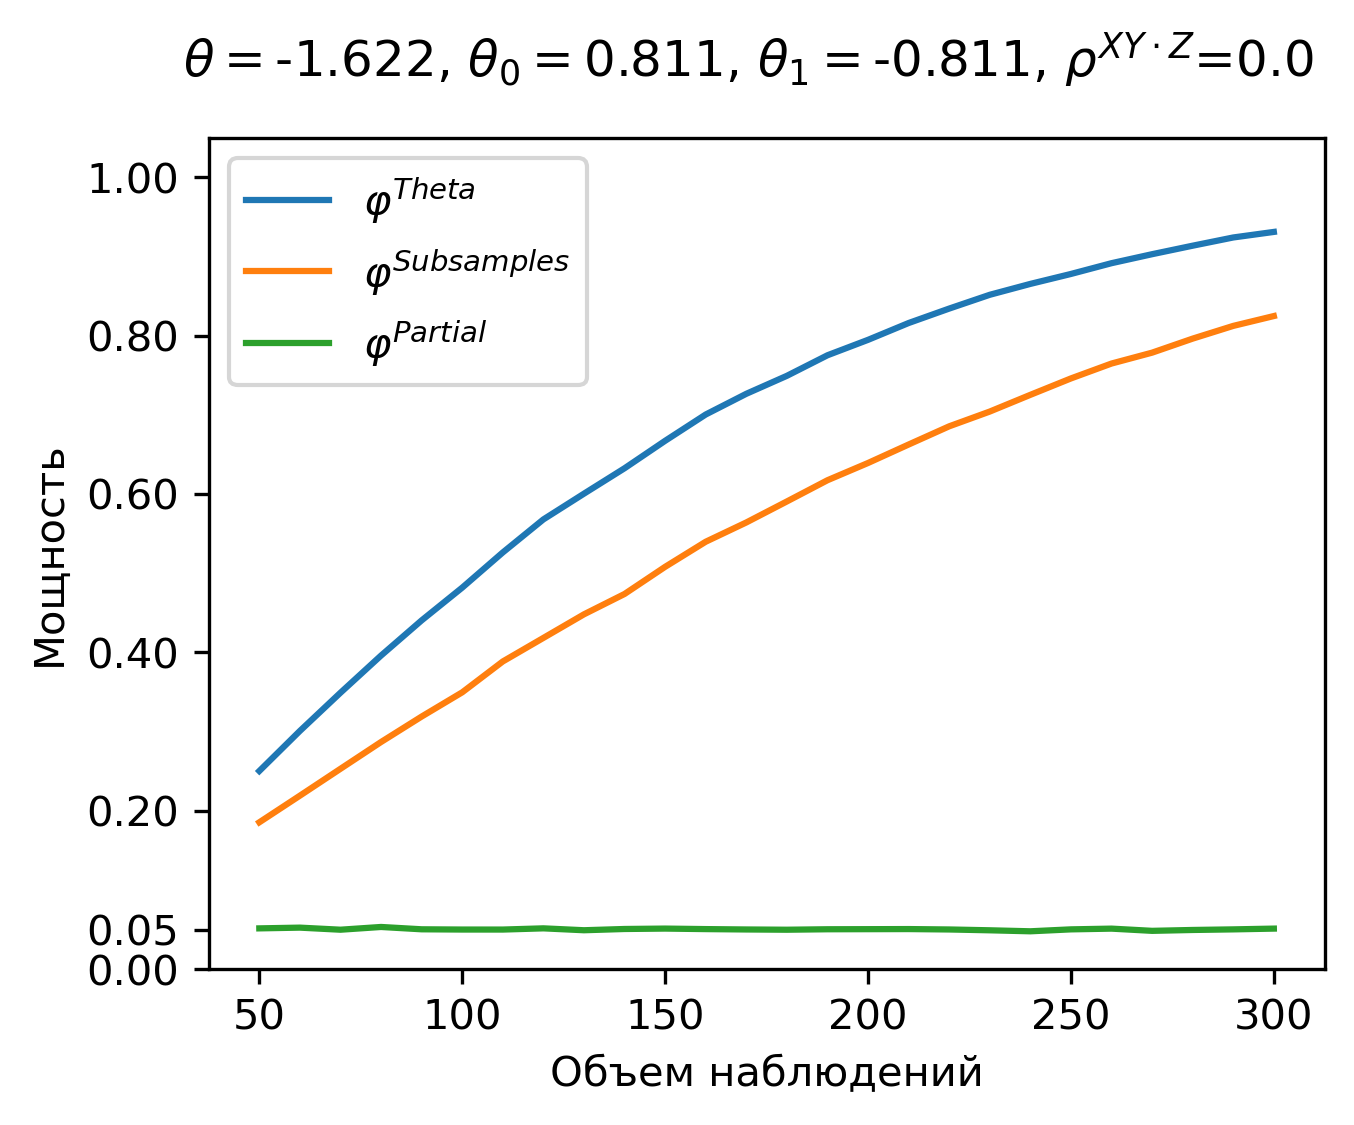
\includegraphics[scale=0.8]{images/graph4.png}
    \caption{Графики зависимости мощности от количества наблюдений
    на тестах $\varphi^{\text{$\theta$-UMPU}}$, $\varphi^{\text{Subsamples}}$, $\varphi^{\text{Partial}}$
    в трехмерном распределении Бернулли с $p_{000}=0.15, p_{001}=0.1, 
    p_{010}=0.1, p_{011}=0.15,
    p_{100}=0.1, p_{101}=0.15, p_{110}=0.15, p_{111}=0.1$. Вероятности оцениваются по $10^5$ экспериментам.} \label{fig:4}
\end{figure}

\begin{figure}[H]
    \centering
    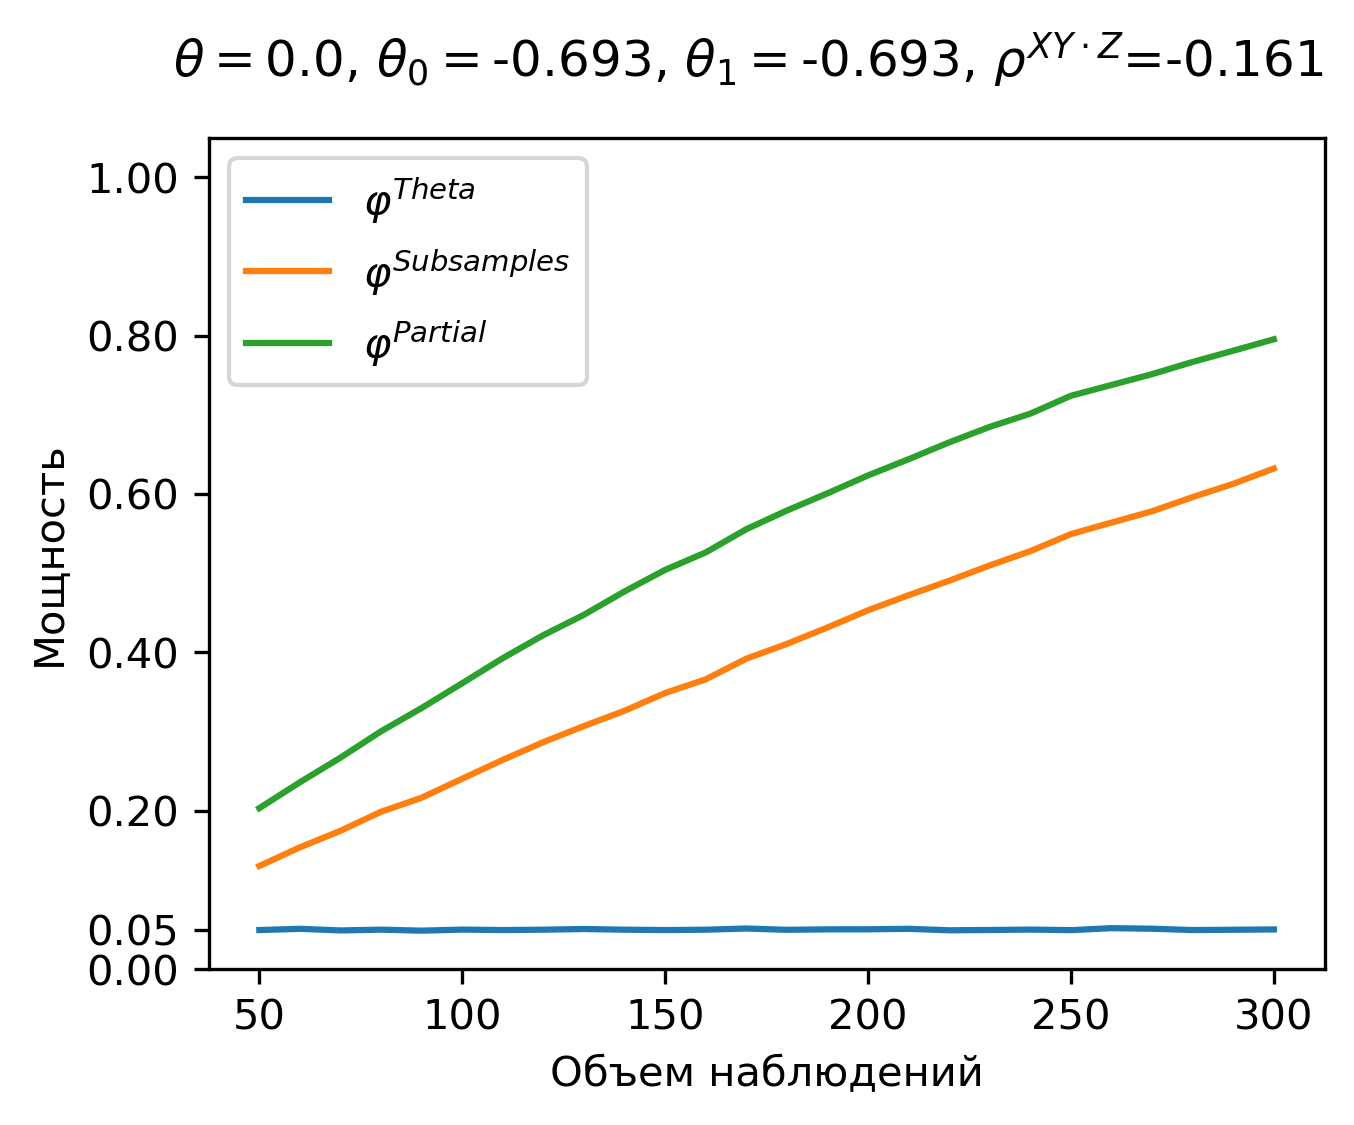
\includegraphics[scale=0.8]{images/graph5.png}
    \caption{Графики зависимости мощности от количества наблюдений
    на тестах $\varphi^{\text{$\theta$-UMPU}}$, $\varphi^{\text{Subsamples}}$, $\varphi^{\text{Partial}}$
    в трехмерном распределении Бернулли с $p_{000}=0.15, p_{001}=0.05, 
    p_{010}=0.3, p_{011}=0.1,
    p_{100}=0.1, p_{101}=0.1, p_{110}=0.1, p_{111}=0.1$. Вероятности оцениваются по $10^5$ экспериментам.} \label{fig:5}
\end{figure}

\begin{figure}[H]
    \centering
    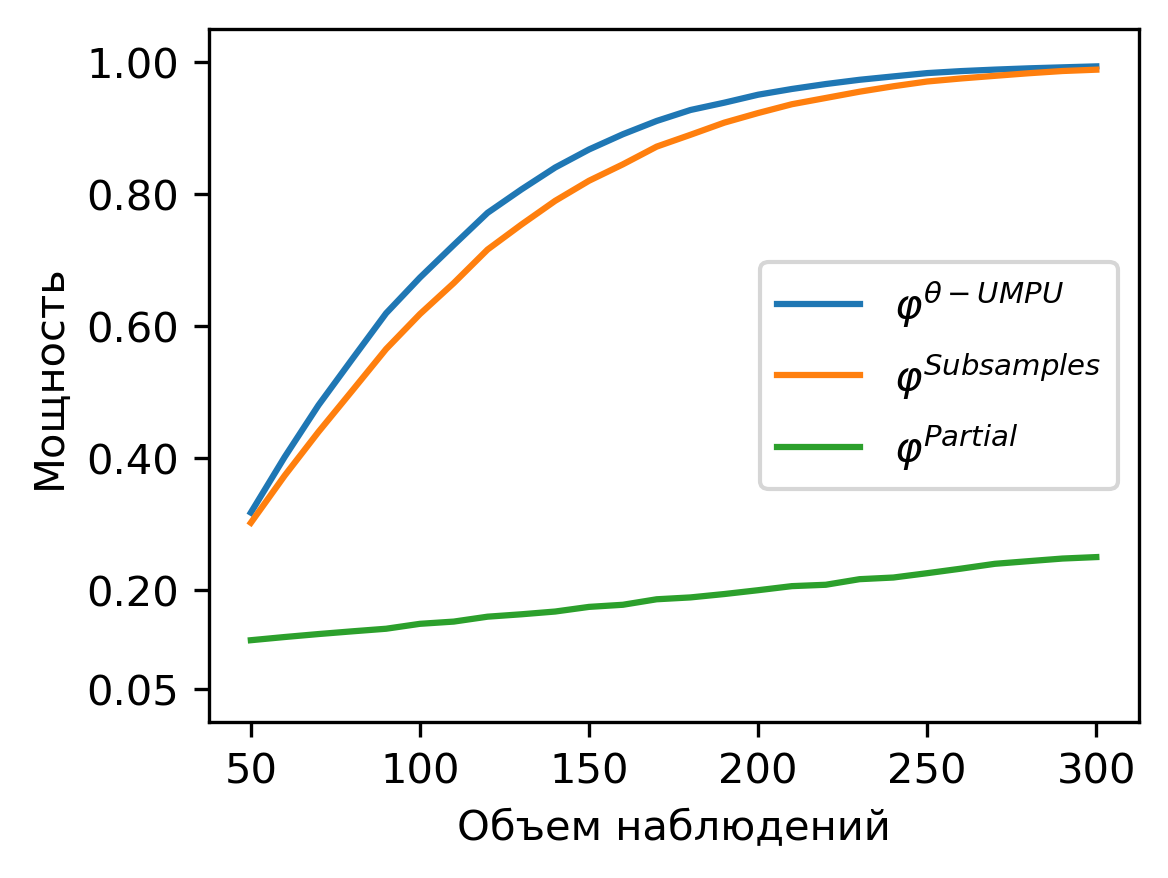
\includegraphics[scale=0.8]{images/graph6.png}
    \caption{Графики зависимости мощности от количества наблюдений
    на тестах $\varphi^{\text{$\theta$-UMPU}}$, $\varphi^{\text{Subsamples}}$, $\varphi^{\text{Partial}}$
    в трехмерном распределении Бернулли с $p_{000}=0.03, p_{001}=0.1, 
    p_{010}=0.04, p_{011}=0.08,
    p_{100}=0.3, p_{101}=0.1, p_{110}=0.07, p_{111}=0.28$. Вероятности оцениваются по $10^5$ экспериментам.} \label{fig:6}
\end{figure}

\begin{figure}[H]
    \centering
    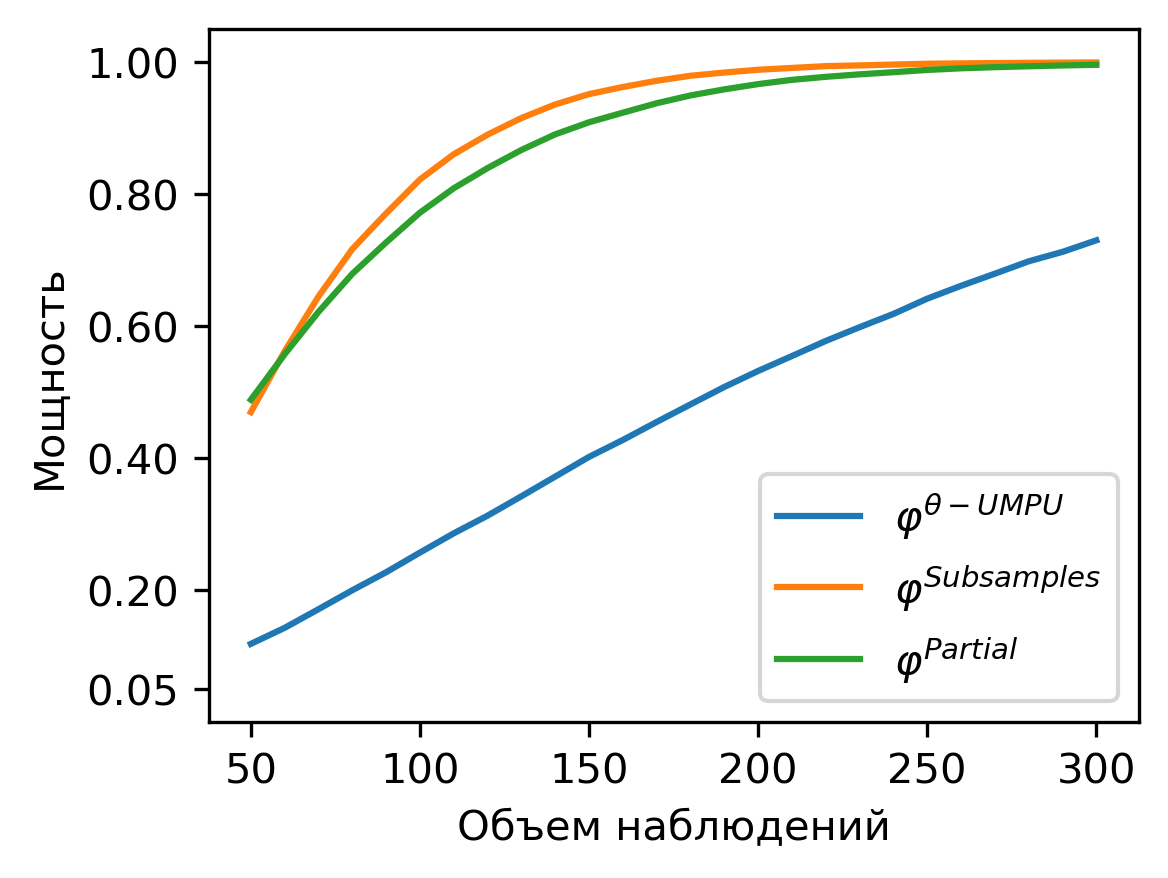
\includegraphics[scale=0.8]{images/graph7.png}
    \caption{Графики зависимости мощности от количества наблюдений
    на тестах $\varphi^{\text{$\theta$-UMPU}}$, $\varphi^{\text{Subsamples}}$, $\varphi^{\text{Partial}}$
    в трехмерном распределении Бернулли с $p_{000}=0.21, p_{001}=0.12, 
    p_{010}=0.04, p_{011}=0.34,
    p_{100}=0.1, p_{101}=0.12, p_{110}=0.02, p_{111}=0.05$. Вероятности оцениваются по $10^5$ экспериментам.} \label{fig:7}
\end{figure}
